\documentclass{article} % say
\usepackage{tikz}
\pagestyle{empty}
\begin{document}
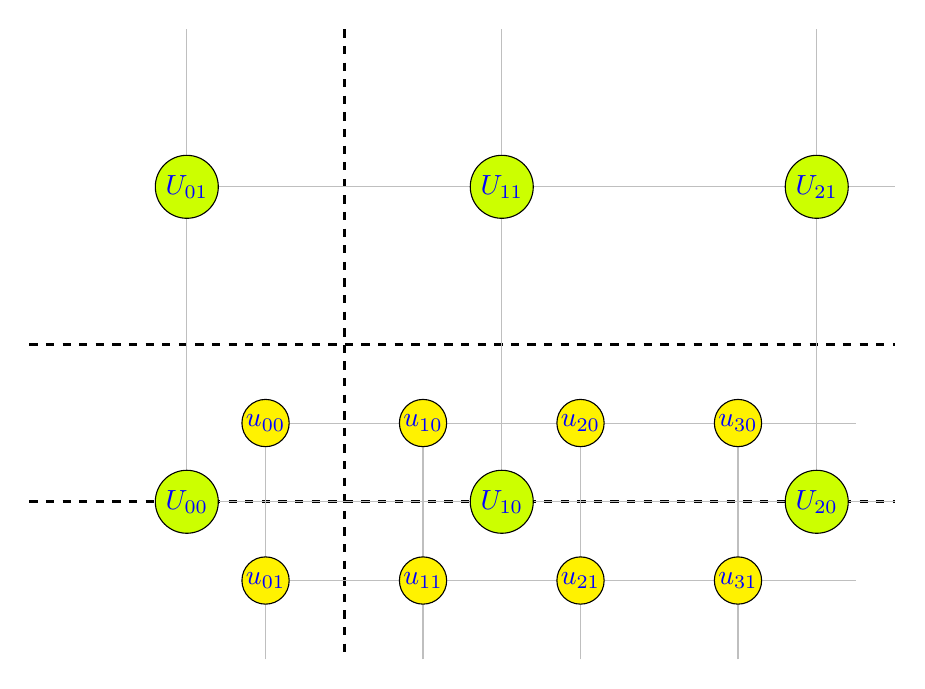
\begin{tikzpicture}
\draw[black, dashed,very thick](0,4)--(0,-4) (-4,0)--(7,0) (-4,-2)--(7,-2);
\draw[gray!50, step=4cm, xshift=-2cm, yshift=-2cm] (0,0) grid (9,6);
\draw[gray!50, step=2cm, xshift=-1cm, yshift=-1cm] (0,-3) grid (7.5,0);

\foreach \x/\y/\z in {0/0/00,1/0/10,2/0/20,3/0/30,0/-1/01,1/-1/11,2/-1/21,3/-1/31} \filldraw[fill=yellow] (-1,-1)+(\x*2,\y*2)circle (.3cm) node[blue]{$u_{\z}$};

\foreach \x/\y/\z in {0/0/00,1/0/10,2/0/20,0/1/01,1/1/11,2/1/21} \filldraw[fill=green!20!yellow] (-2,-2)+(\x*4,\y*4)circle (.4cm) node[blue]{$U_{\z}$};


\end{tikzpicture}

\end{document}
 
